\section{Introduction}\label{sec:intro}

Does it cost energy to shift the phase of a wave? At a single frequency the
answer is no. A delay line of length $\tau$ multiplies a wave of angular
frequency $\omega$ by $e^{i\omega\tau}$, and by choosing $\tau$ one obtains any
phase at all, without loss.\footnote{The factor $e^{i\omega\tau}$ is periodic in $\tau$ with period $2\pi/\omega$, so a delay of at most one period gives every phase; at $5$\,MHz one degree takes $555.6$\,ps (\cref{sec:audit}).} The question becomes interesting only when the
same phase shift is asked of every frequency in a band. A delay cannot do
that, because its phase grows linearly with frequency. A system that does it
moves the oscillations of a pulse under a fixed envelope, which is what one
means by a phase shift of a signal rather than of a single sinusoid
(\cref{fig:pulses}).

This paper answers the question for that case. It was raised in an earlier
paper by one of us with S.~N. Thakur \cite{tb23,tb23pre}, where a $1^\circ$
phase shift of a 5\,MHz wave was assigned a delay of $555$\,ps and an
``infinitesimal energy loss'' $\Delta E=hf\Delta t$. The delay is right; the
energy formula is not (\cref{sec:audit}). It has the units of an action, its
numerical value in \cite{tb23} is off by nine orders of magnitude, and a fixed
phase shift changes neither the frequency nor the energy of a wave. What
survives is the intuition behind it, that a phase shift has an energy price,
and that intuition turns out to be correct in a precise and sharp form once
the shift is required on a band.

\subsection{The result}

We work with causal, time-invariant, passive systems, described by a
transfer function $H$ that is analytic and bounded by $1$ in the upper
half-plane $\Cp$, with real impulse response. With the convention that a pure
delay is $e^{i\omega\tau}$, the phase $\varphi(\omega)$ of $H$ is a lag when it
is positive, and $\alpha(\omega)=-\log\abs{H(\omega)}\ge0$ is the attenuation
in nepers.\footnote{An amplitude attenuation of one neper is $20/\ln10\approx8.686$\,dB, and the power transmission is $\abs{H}^2=e^{-2\alpha}$.} We call $H$ \emph{zero-free} when it has no zeros in $\Cp$; this
class contains the minimum-phase systems, every system $e^{ih}$ with $h$ a
passive response function, and the lossless resonances of Foster
\cite{foster}.\footnote{Foster's reactance theorem: the impedance of a lossless one-port, as a function of $z=\omega$, is an odd Herglotz function, so its reactance increases with frequency between consecutive poles. The corresponding transfer factors $e^{ih}$ have $\abs{H}=1$ on the real axis off the poles of $h$.} Our main theorem (\cref{thm:main}) reads as follows.

\begin{quote}
\emph{Let $H$ be zero-free and passive, continuous and nonzero near the band
$[a,b]$, $0<a<b$, and suppose that its phase on the band is
$\varphi(\omega)=\theta+\tau\omega$ with $\theta\ge0$ and any $\tau\in\R$. Then}
\begin{equation}\label{eq:intro-main}
\frac1{b-a}\int_a^b\alpha(\omega)\dd\omega\;\ge\;\theta\,\Lambda,
\qquad
\Lambda=\frac{K(\kappa)-E(\kappa)}{\kappa},
\end{equation}
\emph{where $\kappa=(b-a)/(b+a)$ and $K,E$ are the complete elliptic
integrals. Equality holds if and only if the system has no response outside
the band, in a sense made precise by its Herglotz measure, and it is attained
by an explicit system $H_\star$.}
\end{quote}

The constant is elementary to estimate. Its power series has positive
coefficients and
\begin{equation}\label{eq:intro-bounds}
\begin{gathered}
\frac\pi4\,\kappa\;<\;\Lambda\;\le\;\frac\pi4\,\frac{\kappa}{1-\kappa^2},\\
\Lambda\sim\tfrac12\log\frac{4b}{a}-1\quad(a/b\to0),
\end{gathered}
\end{equation}
so for a narrow band of relative width $\Delta f/f$ a phase shift of one
degree costs at least $1-e^{-2\theta\Lambda}$, about
$(\pi^2/720)\,\Delta f/f\approx0.0137\,\Delta f/f$, of the power at the worst
frequency,\footnote{For a narrow band $\kappa\approx\frac12\Delta f/f$, so $\Lambda\approx\frac\pi4\kappa\approx\frac\pi8\frac{\Delta f}f$; one degree is $\pi/180$ radian, and $1-e^{-2\theta\Lambda}\approx2\theta\Lambda=2\cdot\frac\pi{180}\cdot\frac\pi8\frac{\Delta f}f=\frac{\pi^2}{720}\frac{\Delta f}f$ (\cref{prop:energy}(iv)).} and the same fraction in the geometric mean over the band (\cref{cor:worst,sec:energy}). For an octave the bound is
$0.0415$\,dB per degree, for a decade $0.143$\,dB per degree\footnote{These are $\Lambda\cdot\frac\pi{180}\cdot\frac{20}{\ln10}$ with $\Lambda=0.27353$ for $b/a=2$ and $\Lambda=0.94478$ for $b/a=10$.}
(\cref{tab:lambda}).

Five features of the theorem deserve to be named at once.

\emph{Delay is free.} The term $\tau\omega$ does not enter the bound.\footnote{The reason is the vanishing first moment $\int_a^b\omega\,p(\omega)\dd\omega=0$ of the weight $p$ in \eqref{eq:intro-sum}, \cref{lem:moments}(i).} A
system may delay the envelope by any amount; what it pays for is the
carrier--envelope offset $\theta$ (\cref{prop:cep}).

\emph{The bound is sharp.} The extremal system $H_\star$ of
\cref{thm:extremal} is given by an abelian integral,
\begin{gather*}
H_\star(z)=\exp\Big(i\tau_\star\int_0^z\frac{s^2-m^2}{R(s)}\dd s\Big),\\
R(s)^2=(s^2-a^2)(s^2-b^2),
\end{gather*}
with $m^2=b^2E(k)/K(k)$ and $\tau_\star=2\theta K(k)/(\pi b)$,
$k^2=1-a^2/b^2$. It is lossless outside the band, its attenuation vanishes at
both band edges and peaks at $\omega=m$, and its phase is exactly $\theta$
across the band (\cref{fig:extremal}).

\emph{Lossless resonances make things worse.} A reactive element resonating
outside the band, the classical device for shaping phase, contributes a
strictly positive term to the loss (\cref{rem:resonances}). A lossless system
cannot have a constant phase on any band unless it is $\pm1$
(\cref{cor:rigid}).

\emph{Phase leads obey the mirror bound.} If $\theta<0$ the same
inequality holds for the mean of $\alpha$ weighted by $ab/\omega^2$
(\cref{thm:lead}), so the worst frequency of a system whose phase is constant
modulo $2\pi$ loses at least $\dist(\theta,\pi\Z)\,\Lambda$ nepers
(\cref{cor:worst}).

\emph{Zeros help, by an amount we determine exactly.} For
$0<\theta<a\pi/(a+b)$ a single zero on the imaginary axis already lowers the
attainable mean attenuation strictly below the least value among all
zero-free systems with the same argument (\cref{prop:onezero,cor:zerosbeat}).
The least loss over all passive systems, with any zeros, is the subject of
our second theorem.

\subsection{Systems with zeros}

Once zeros are allowed, $\log H$ is no longer defined and the sum rule
does not apply. We pass instead to $\zeta=\log F$, where
$F=e^{-i\theta}(H-e^{i\theta})/(H-e^{-i\theta})$ maps the values of $H$ into the
upper half-plane. Zeros of $H$ become ordinary values of $\zeta$, the phase
condition becomes the condition that $\zeta$ lies on a fixed curve over the
band, and a comparison argument in Hardy spaces gives a bound at every
frequency (\cref{thm:allzeros}).

\begin{quote}
\emph{Let $0<\theta<\pi$. There is a passive system $\Hs_\theta$, with one zero,
on the imaginary axis, and lossless off the band, such that every passive
system $H$ that is continuous and nonzero near the band and has
$\arg H\equiv\theta$ modulo $2\pi$ there satisfies
\[
\alpha(\omega)\ \ge\ \as_\theta(\omega)\qquad(a\le\omega\le b),
\]
where $\as_\theta$ is the attenuation of $\Hs_\theta$, with equality on a set of
positive measure only for $H=\Hs_\theta$.}
\end{quote}

The optimal system is $-B_{\eta_\star}e^{ih}$, a single Blaschke factor times a
zero-free system, where the zero $i\eta_\star$ is fixed by the condition that
the zero-free factor has no delay at high frequency. The minimal mean is
$\theta\Lambda$ minus an explicit integral, it is positive, and this answers
\cref{prob:zeros}. For a right angle the optimal system is algebraic
(\cref{thm:rightangle}),
\[
\Hs_{\pi/2}(z)=-\frac{z^2+ab}{R(z)+i(a+b)z},
\]
its mean attenuation is $\frac\pi2(\sqrt b-\sqrt a)/(\sqrt b+\sqrt a)$, and its
attenuation peaks at the geometric centre with the value $\frac12\log(b/a)$.
So no passive system whose phase is a right angle at every frequency of an
octave transmits more than half of the power at $\omega=\sqrt{ab}$: the loss
there is at least $3.01$\,dB, and for a decade at least $10$\,dB. For a
narrow band the least mean loss with zeros is
$\frac\pi8\sin\theta\,\Delta f/f$, against $\frac\pi8\theta\,\Delta f/f$ without
(\cref{cor:narrowzeros}); small phase shifts gain almost nothing from zeros.

\subsection{How the theorem is proved}

The proof rests on a single identity. If $H=\pm e^{ih}$ with $h$ a Herglotz
function, then for every band
\begin{equation}\label{eq:intro-sum}
\int_a^b\alpha\dd\omega
=\frac12\int_a^b\varphi(\omega)\,p(\omega)\dd\omega
+\frac\pi4\int_{\R\setminus S}W\dd\mu ,
\end{equation}
where $S=[-b,-a]\cup[a,b]$, $\mu$ is the Herglotz measure of $h$, and
\begin{gather*}
p(\omega)=\frac{a^2+b^2-2\omega^2}{\sqrt{(\omega^2-a^2)(b^2-\omega^2)}},\\
W=\frac{(\rho-1)^2}{\rho},\qquad
\rho(z)=\sqrt{\frac{z^2-a^2}{z^2-b^2}} .
\end{gather*}
The function $W$ is analytic in $\Cp$, its real part equals $-2$ on the band
and is strictly positive on the rest of the real line, and its imaginary part
is $p$ on the band (\cref{fig:testfunction}). The identity
\eqref{eq:intro-sum} then follows from the Kramers--Kronig relations
\cite{kronig,kramers,toll} in their Herglotz form. Since $\int_a^b\omega
p\dd\omega=0$, a delay drops out; since $\int_a^bp\dd\omega>0$ and the last
term is nonnegative, a positive constant phase forces loss. The value of
$\int_a^bp\dd\omega$ is an elliptic integral, which a Landen transformation
brings to the form \eqref{eq:intro-main}.

Sum rules of this kind have a long history. Bode's gain--phase relations
\cite{bode} bound the phase of a minimum-phase system by its gain; Fano
\cite{fano} bounded the bandwidth of impedance matching; Rozanov
\cite{rozanov} bounded the thickness of absorbers; and Gustafsson, Sj\"oberg,
Bernland and Luger \cite{gustafsson,bernland} turned the Herglotz
representation into a general machine for physical bounds. Miller
\cite{miller} bounded the delay--bandwidth product of slow light. The
inequality \eqref{eq:intro-main} is, to our knowledge, new: we did not find a
bound on the loss forced by a frequency-independent phase shift in this
literature, nor in the work on broadband phase shifters, where constant
phase \emph{differences} between two lossless channels are realised
\cite{darlington} and constant absolute phase is not attempted. The test
function $W$, which is tailored to an affine phase, is what makes the bound
sharp.

\subsection{What the result is, and what it is not}

The theorem is a sharp inequality of classical analysis with a direct
physical reading: a carrier--envelope phase shift over a band has a minimal
price in absorbed energy, proportional to the shift and, for narrow bands,
to the relative bandwidth. It is not a statement about energy conservation:
a constant phase factor is energy neutral (\cref{prop:static}), and the price
is paid because causality and passivity tie the phase of $H$ on the band to
its modulus everywhere. Nor does it rest on quantum mechanics; when the wave
is quantised, the bound becomes a lower bound on the probability that a
quantum in the band is absorbed (\cref{sec:energy}). The energy $hf$ of a
quantum, which played the main part in \cite{tb23}, enters only through the
kinematics of frequency shifts in \cref{sec:kinematics}; see also
\cite{tbf23,tb23cosmic,bh22} for other uses of the photon energy by the
first author and coworkers.

\subsection{Plan}

\Cref{sec:audit} checks the equations of \cite{tb23}.
\Cref{sec:kinematics} separates the three things a ``phase shift'' can mean:
a constant factor, a delay, and a phase that changes in time.
\Cref{sec:passive} sets up passive systems and their Herglotz functions, and
\cref{sec:test} constructs the test function. The sum rule and the main
theorem are in \cref{sec:sumrule}, the evaluation of the constant in
\cref{sec:constant}, the extremal systems in \cref{sec:extremal}, and the
effect of a single zero in \cref{sec:zeros}; \cref{sec:allzeros} finds the
least loss over all passive systems. \Cref{sec:waves} applies the results to
waves in passive media and returns to the 5\,MHz example.
\Cref{sec:discussion} lists open problems. \Cref{fig:roadmap} shows how
the results depend on each other. \Cref{app:elliptic} derives, from the
series alone, every fact on complete elliptic integrals that is used
(Legendre's relation, the invariance of the arithmetic--geometric mean and
Landen's transformations); \cref{app:integrals} computes the integrals of the
weight; \cref{app:profiles} derives the formulas for the extremal profile;
and \cref{app:verification} describes what has been checked by machine.
Every statement is proved in the text. The finite and algebraic parts of the
proofs (dimensional analysis, the coefficient recurrences, enclosures of
$\Lambda$ and the polynomial identities) are certified in Lean~4, and a
script re-evaluates every numerical value.

\begin{figure}[t]
\centering
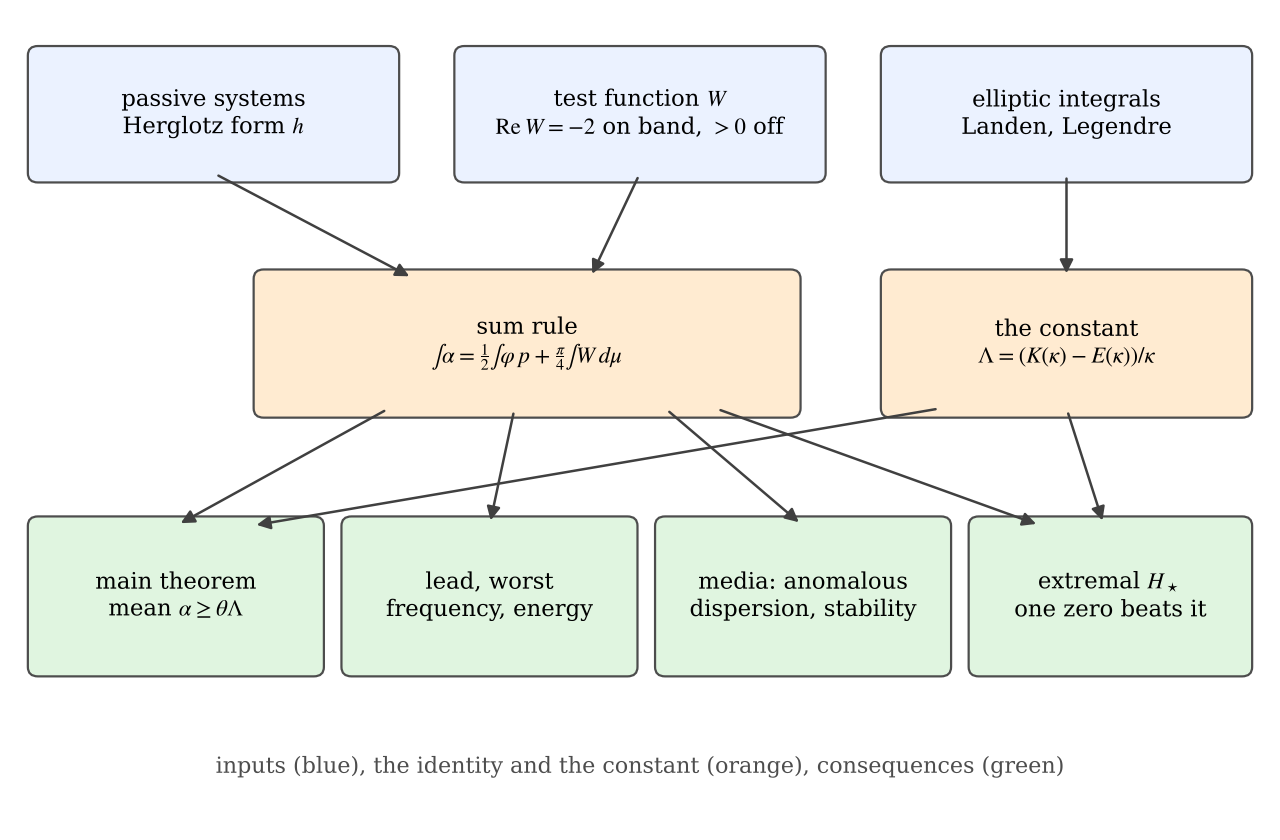
\includegraphics[width=\columnwidth]{figures/fig_roadmap.png}
\caption{How the results depend on each other. The sum rule
(\cref{thm:sumrule}) is built from the test function $W$ (\cref{sec:test});
the constant $\Lambda$ comes from the moments of the weight
(\cref{sec:constant}); every later statement is a consequence of these two
or of the extremal system of \cref{thm:extremal}.}
\label{fig:roadmap}
\end{figure}

\begin{figure}[t]
\centering
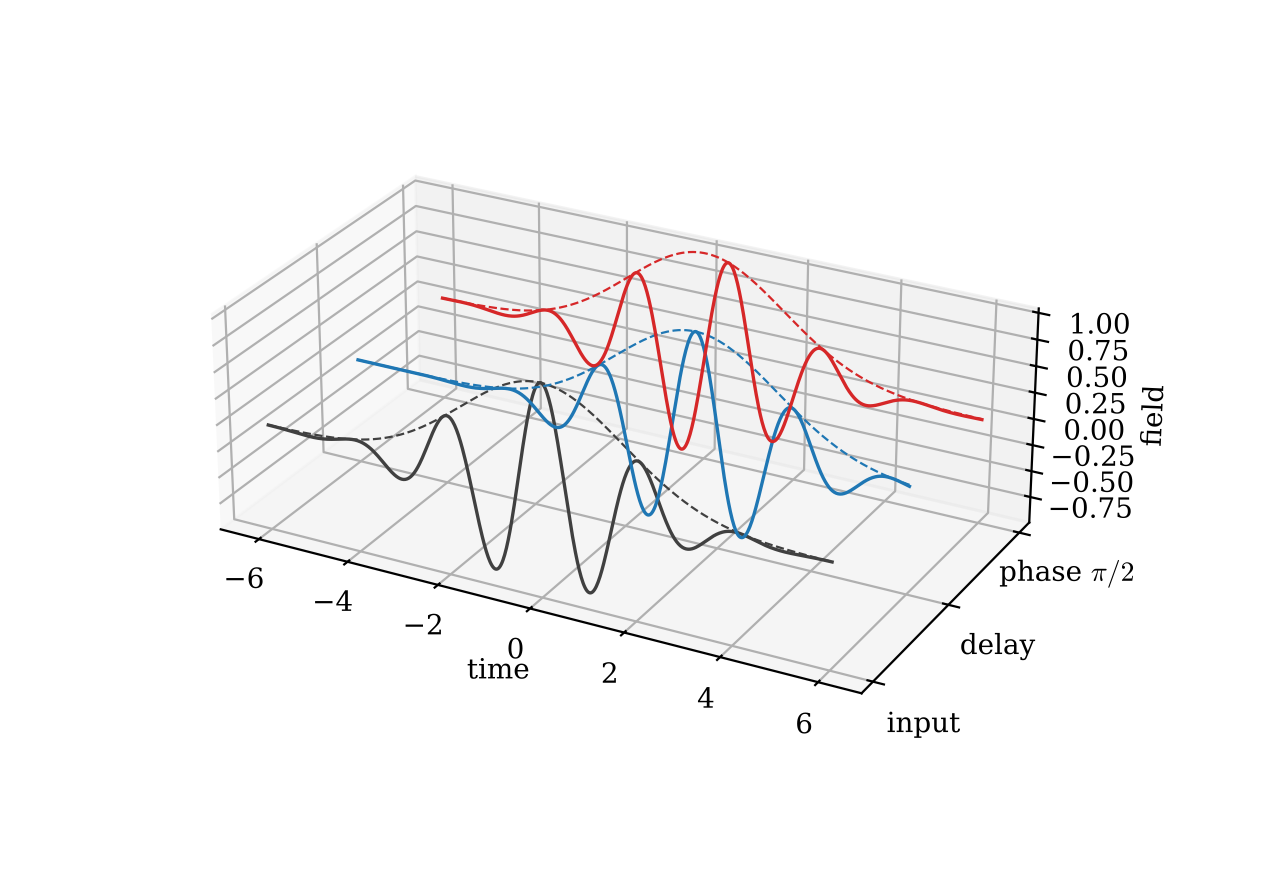
\includegraphics[width=\columnwidth]{figures/fig_pulses.png}
\caption{A pulse (grey), the same pulse after a delay (blue), and after a
constant phase shift of $\pi/2$ on its whole band (red). Dashed curves are the
envelopes. The delay moves the envelope and the oscillations together; the
constant phase shift moves the oscillations under a fixed envelope. Only the
second operation costs energy in a passive system.}
\label{fig:pulses}
\end{figure}
